\documentclass[10pt,twocolumn,letterpaper]{article}

\usepackage{cvpr}
\usepackage{times}
\usepackage{epsfig}
\usepackage{graphicx}
\usepackage{amsmath}
\usepackage{amssymb}

% Include other packages here, before hyperref.
\usepackage{tabularx} % in the preamble
\newcolumntype{Y}{>{\centering\arraybackslash}X}
\newcommand\VRule[1][\arrayrulewidth]{\vrule width #1}
\usepackage{array,booktabs,arydshln,xcolor} % for widening table line
\usepackage{amsthm,bm}
\usepackage{epstopdf}


\usepackage{amsthm}
\usepackage{multirow}

\usepackage{float}
\usepackage{wrapfig}
\usepackage{subcaption}
\usepackage{capt-of}% or \usepackage{caption}
\usepackage{booktabs}
\usepackage{varwidth}

\usepackage{algpseudocode,algorithm,algorithmicx}
\newcommand*\DNA{\textsc{dna}}

\newcommand*\Let[2]{\State #1 $\gets$ #2}
\algrenewcommand\algorithmicrequire{\textbf{Precondition:}}
\algrenewcommand\algorithmicensure{\textbf{Postcondition:}}


\makeatletter
\def\BState{\State\hskip-\ALG@thistlm}
\makeatother

\usepackage{bm}

\usepackage[breaklinks=true,bookmarks=false]{hyperref}

%\cvprfinalcopy % *** Uncomment this line for the final submission

\def\cvprPaperID{****} % *** Enter the CVPR Paper ID here
\def\httilde{\mbox{\tt\raisebox{-.5ex}{\symbol{126}}}}

% Pages are numbered in submission mode, and unnumbered in camera-ready
%\ifcvprfinal\pagestyle{empty}\fi
%\setcounter{page}{4321}
\begin{document}

%%%%%%%%% TITLE
\title{Semantic High-definition Image Synthesis \\ with a Hierarchically-nested Adversarial Network}

\author{First Author\\
Institution1\\
Institution1 address\\
{\tt\small firstauthor@i1.org}
% For a paper whose authors are all at the same institution,
% omit the following lines up until the closing ``}''.
% Additional authors and addresses can be added with ``\and'',
% just like the second author.
% To save space, use either the email address or home page, not both
\and
Second Author\\
Institution2\\
First line of institution2 address\\
{\tt\small secondauthor@i2.org}
}

\maketitle
%\thispagestyle{empty}

%%%%%%%%% ABSTRACT
\begin{abstract}
This paper presents a novel and effective method to deal with the challenging task of generating synthetic photographic image conditioned on semantic image descriptions. We show a fully end-to-end trainable network that can generate high resolution images (e.g. $512^2$).
Our method leverages the deep representations of convolutional layers and introduces hierarchical-nested adversarial training to regularize the representations and capture the complex image statistics. We present a new network architecture, which is intuitive as well as extensile, to push generated images to high resolutions. \textcolor{red}{We present a functional generative adversarial networks (GANs) training strategy} to encourage more effective multimodal (i.e. image and text) information utilization in order to enhance multi-purpose adversary between real and fake distribution. 
With extensive experimental validation on three major datasets, our method significantly improves previous state of the arts. 

\end{abstract}


%%%%%%%%% BODY TEXT
\section{Introduction}
Generating photographic image conditional on arbitrary semantic description is an important problem in generative model research \cite{reed2016generative}. However, insufficient methods have been successfully developed to address this task due to its particular challenges. Text-to-image synthesis can be viewed as an special variation of conventional generative models, which aim to translate a low-dimensional embedding  to a much more complex RGB image space.  Differently, the embedding space of the former is induced by semantic descriptions. Therefore, this task requires the generated images to be \textit{semantically consistent}, i.e., the generated images not only preserve sketch concepts of descriptions generally but also preserve fine-grained descriptive details in image pixels. 

Generative adversarial networks (GANs) have become the main solution to this task. 
Reed \etal \cite{reed2016generative} is th first to address this task through a GAN based framework. But this method only handles image up to $64{\times}64$ resolution and usually can barely generate vivid object details.
Based on this method, Zhang \etal \cite{han2017stackgan} present a successful approach (StackGAN) by stacking another GAN to generate high-quality $256{\times}256$ images given low resolution $64{\times}64$ synthetic images. This method needs two-stage training to achieve the goal. Later on, Dong \etal \cite{dong2017semantic} 
bypasses the difficult of translate vector embedding to RGB images and treat it as an pixel-to-pixel translation \cite{isola2016image}, by re-rendering an arbitrary-style training ($128{\times}128$) image conditioned on a targeting semantic description. Unfortunately, its high resolution synthesis ability is still unclear. 
At present, how to train from the low-dimensional text space to synthesize high resolution and diverse images in an end-to-end manner is still an open and attractive question. 

We outline several empirical reasons for this challenges using GANs to deal with text-to-image synthesis. The first comes from a fundamental difficulty of balancing the convergence between generators and discriminators \cite{goodfellow2014generative,improvedGAN}. How to utilize the multimodal information between images and text in discriminator is extremely important to generate effective gradients. The second is that huge pixel space in high resolution images \cite{han2017stackgan}. 
An effective regularization to regularize generators is critical to help capture the complex image statistics \cite{huang2016stacked} as well as preserve semantic consistency. 
%The first reason is that the pixel space in high resolution image is substantially large \cite{han2017stackgan}. 
% Keeping semantic consistency as well as diversity
%The first reason comes from the fundamental difficulty of balancing the stability between generators and discriminators. There are a rich number of literature trying to stabilize GAN training \cite{salimans2016improved} and regularize networks \cite{huang2016stacked}. 
%But especially for text-to-image synthesis, how to utilize the multimodal information between images and text in discriminator is extremely important and needs careful consideration. The second reason is that the pixel space in high resolution image is substantially large \cite{han2017stackgan}. Keeping semantic consistency as well as diversity in generated images needs more specialized designs for discriminators to generate effective gradients, as well as generators to prevent gradient vanishing. 
With careful consideration of these outlined problems, in this paper, we propose a novel fully end-to-end method that can directly model high resolution image statistics and generate semantic consistent and photographic image up to $512^2$ resolution. The contributions are described follows.

Our generator is a simple Vanilla GAN, without needing any inside text conditioning \cite{han2017stackgan} or image label supervision \cite{dash2017tac}. To tackle the problem of the big leap from the text space to the high resolution image space, our insight is to leverage hierarchical representations with additional implicit constraints to reduce training instability. 
We introduce ``accompanying'' hierarchically-nested adversarial objective at intermediate layers to generate multi-scale images.  
And we present an generator network structure design than can uses gradients from multi-scale nested discriminators more effectively.

To better make use of image and text information in GAN training, 
\textcolor{red}{we enforce discriminators at different resolutions can simultaneously differentiate real and fake image-text pairs, images, and patches.}
This multi-purpose conditional adversary is mutually beneficial to encourage each only focuses on respect duties. 
%It is a regularization to limit the discriminators to use unexpected information to make decision. 
We validate our proposed method on three datasets, i.e. CUB birds \cite{welinder2010caltech}, Oxford-102 flowers \cite{Nilsback08}, and large-scale COCO datasets \cite{lin2014microsoft}. Extensive experimental results and analysis demonstrate the effectiveness of our method and significantly improved performance compared against previous state of the arts. All source code will be released.


\section{Related Work}
We discussed related methods as well as clarify the novelty of our method.

Deep generative models grows wide interests recently, including GANs \cite{goodfellow2014generative}, Variational Auto-encoders (VAE) \cite{kingma2013auto}, etc \cite{oord2016pixel}. 
There are substantial existing methods investigating better usage of GANs for different applications, such as image synthesis \cite{radford2015unsupervised, shrivastava2016learning}, (unpaired) pixel-to-pixel translation \cite{isola2016image,zhu2017unpaired}, medical applications \cite{costa2017towards}, etc \cite{ledig2016photo,huang2016stacked}.

Text-to-image synthesis not only requires diverse and high-quality generation but also requires precise semantically consistent mapping in the image space.  Reed \etal \cite{reed2016generative} introduce a method that can generate $64{\times}64$ resolution images, which is similar with DCGAN \cite{radford2015unsupervised}. This method presents a new strategy to image-text matching aware adversarial training. Reed \etal \cite{reed2016learning} propose generative
adversarial what-where network (GAWWN) to enable "where and what" instructions in text-to-image synthesis, which uses extra information to help generate $128{\times}128$ resolution images. StackGAN \etal \cite{han2017stackgan} propose to a two-stage stacking GAN training approach that is able to generate $256{\times}256$ compelling results. Recently, Dong \etal \cite{dong2017semantic} propose to learn a joint embedding of images and text so as to re-render a prototype image conditioned on targeting descriptions. Cha \etal \cite{char2017perceptual} explore the usage of the perceptional loss with a pretrained ImageNet CNN \cite{johnson2016perceptual} and Dash \etal \cite{dash2017tac} make use of auxiliary classifiers (similar with \cite{odena2016conditional}) to assist GAN training. 
	
Learning a continuous mapping from low-dimensional embeddings to complex real data distribution is a long-standing problem. Although GANs have made significant progressive, there are still many  unsolved difficulties, e.g. training instability and high resolution. Wide methods have been proposed to address those tasks, through various stabilization training techniques \cite{salimans2016improved,arjovsky2017wasserstein,berthelot2017began,shrivastava2016learning,odena2016conditional}, regularization using outside knowledge (e.g. image labels, ImageNet CNNs, etc) \cite{dosovitskiy2016generating,ledig2016photo,dash2017tac,dash2017tac}, or multiple discriminators  \cite{metz2016unrolled,durugkar2016generative,yang2017lr}. While note that our method does not use any extra information apart from training paired text and images. Moreover, it is easy to see the training difficulty grows significantly as targeting image resolution increases.

%for example, label smoothing and discriminator feature matching \cite{salimans2016improved, }, training stronger discriminator is beneficial to encourage generators \cite{arjovsky2017wasserstein}. Balancing through a equilibrium enforcing method \cite{berthelot2017began}
%Preventing discriminators from forgetting past samples and re-introduces artifacts \cite{shrivastava2016learning}. Increasing the information richness in GANs has been shown very useful \cite{odena2016conditional}.  

To synthesize high resolution images, cascade networks play an important role to decompose original difficult tasks to multiple subtasks.
Denton \etal \cite{denton2015deep} trains a cascade of GANs within a Laplacian pyramid framework (LAPGAN) and use each to generate difference images, conditioned on random noises and output from last level of the pyramid, to push up output resolution through by-stage refinement. StackGAN also shares similar strategy with LAPGAN. Following this strategy, Chen \etal \cite{chen2017photographic} present a cascaded refinement networks to synthesis high-resolution scene from semantic maps. 
Huang \etal \cite{huang2016stacked}
shows a top-down stack GAN to leverage mid-level representations, which shares some similarities with StackGAN and our method. However, this method need multiple symmetric  bottom-up discriminators and pre-training of discriminators, and the usage for high-resolution image is unclear \cite{han2017stackgan}. Recently, Karras \cite{} show a progressive training of GANs to enable high resolution image generation. Compared with these strategies that train low- to high-resolution GANs progressively, our method has advantages of utilizing multi-level representations to encourage implicit subtask integration, which enables end-to-end high resolution image synthesis.

%More advantages of our method compared with others will be demonstrated in the following.

Leveraging hierarchical representations of neural networks is an effective way to enhance implicit multi-scaling and ensembling for tasks such as image classification \cite{lee2015deeply} and pixel or object classification \cite{xie2015holistically,cai2016unified,long2015fully}. DSN \cite{lee2015deeply} proposes deep supervision in hierarchical convolutional layers to increase the discriminativeness of feature representations. 
Our method is partially inspired by supervised CNNs with deep supervision \cite{lee2015deeply,xie2015holistically}. Our proposed hierarchically-nested adversarial supervision enhances layer representations to support final high resolution outputs.   
\begin{figure}[t]
	\centering
	%	\includegraphics[width=0.48\textwidth]{}
	\caption{} \label{fig:archs}
\end{figure}

%
%
%
%\subsection{Summarize different architectures}
%refer to HED.
\begin{figure}[t]
	\centering
%	\includegraphics[width=0.48\textwidth]{}
	\caption{} \label{fig:archs-compare}
\end{figure}

\section{Method}
Figure \ref{fig:archs} illustrate the overall method.


\section{Preliminary}
\subsection{Generative Adversary Network}
Generative adversary networks (GANs) are composed of a generator $G$ and a discriminator $D$, which are alternatively trained to compete with each other in a two-player minimax game. The discriminator $D$ is optimized to distinguish the synthesized images from the real images, meanwhile, the generator $G$ is trained to fool the discriminator by trying to convert an input distribution $p_z$ to the true data distribution $p_{data}$. Concretely, the overall training procedure can be analogous to the following two-player min-max game $V(D, G)$, where the optimal $G$ and $D$ can be obtained by 
\begin{equation}
\label{equ:GAN}
\begin{split}
G^*, {D}^* = \arg~\underset{G}{\min}\ \underset{\mathcal{D}}{\max}~ V(D, G)
\end{split}
\end{equation}

%\begin{equation}
%\label{game}
%\begin{split}
%\underset{G}{\min}\ \underset{D}{\max}\ V(D, G) =  &\mathbb{E}_{x\sim p_{data}}[\log D(x)] +  \\
%&\mathbb{E}_{z\sim p_{z}}[\log (1-D(G(z)))]		   
%\end{split}
%\end{equation}
%where $x$ is a real image sampled from the true data distribution $p_{data}$, $z$ is a noise vector usually sampled from some predefined distribution $p_{z}$ (e.g., Gaussian distribution).
%In practice, It's been shown to work better for the generator $G$ to minimizing $-\log(D(G(z)))$ rather than $\log(1-D(G(z)))$, namely, the $\log(D)$ trick.
%In this paper, we replace the negative log likelihood loss with a least square objective\cite{lsgan}. 

Conditioned GAN \cite{isola2016image} is a variation of traditional GAN where both the generator network $G$ and discriminator network $D$ are conditioned on an additional condition vector besides the noise vector. In this paper, we consider the task of training a deep  generative adversarial network conditioned on the embedding of the text descriptions of the images.

\section{Method}
Figure \ref{fig:archs} illustrate the overall method.
%To generate high-resolution photo-realistic images from text embeddings, we propose a simple and effective Hierarchically-nested Generative Adversarial Network.
Our approach is to train both generator and discriminator conditioned on sentence embedding vectors. We leverage functional loss for discriminator and hierarchically nested side outputs as hierarchical supervision for both generator and discriminator to achieve our goal of generating photo-realistic images from text descriptions.  

In general, the generator takes text embedding and random noise vector as input and synthesis images at different scales (e.g, $64\times64$, $128\times128$, $256\times256$). The discriminator, on the other hand, is trying to judge the pair of synthesized images and the corresponding text embedding as fake pairs as well as differentiating the real images from the fake images. $G$ and $D$ are optimized alternatively until converges.


\textbf{Notation } 
We denote the training data set by $S=\{({X}^n, {T}^n),n=1,...,N\}$, where $X^n$ is the $n-$th training image, and $T^n={t^1,...,t^m}$ as $m$ text descriptions corresponds to $X^n$. 

Since we obtain the text embedding vector  using the per-trained char-rnn text encoder provided in \cite{reed2016generative}. For simplicity, we do not differentiate text description and it's corresponding text embedding vector in this paper.  Our goal is to learn a generator $G$ that could produce high resolution images of high visual quality as well as variability giving an input text description $t$.  

The input to $G$ compress input sentence embedding, and one noise input.
Denote the image dimension, text embedding dimension and the dimension of the noise input as $I$, $T$ and $Z$, respectively. Please note that, $G$ has multiple branches and generates multiple images of different sizes. For each image size, we have a distinct discriminator $D$ associated with it. 
%For simplicity, we only describe one image size.  

The generator is denoted $G: \mathcal{R}^{Z}: \times \mathcal{R}^{T}\rightarrow\mathcal{R}^{I}$, the image discriminator $D_{img}: \mathcal{R}^{I}\rightarrow\{0, 1\}$, and the matching-aware pair discriminator $D_{pair}: \mathcal{R}^{I}: \times \mathcal{R}^{T}\rightarrow\{0, 1\}$. 

\textbf{Variational text embedding } Following the practice of \cite{han2017stackgan}, instead of using the plan deterministic non-linear transformation of the original $t$, we obtain the conditional vector $c$ by sampling from a Gaussian distribution $\mathcal{N}(\mu(t), \Sigma(t) )$, in which the mean $\mu(t)$ and the diagonal covariance matrix $\Sigma(t)$ are non-linear transformation of the original text embedding $t$. This type of conditional augmentation technique can be used to inject randomness into the text embedding vector $t$ to mitigate the common problem that conventional conditional GAN training paradigm usually learns to totally ignore the randomness, resulting to collapsing results lacking diversity \cite{reed2016generative}. In addition, using this kind of text embedding makes the input pure stochastic, making it more difficult for the generator to over fit the training data.

\subsection{Hierarchical Deep Supervision}
Directly predicting high resolution synthesized images are challenging, not only because of the difficulties in training but also due to the large variation and instability in the hidden layers.

Our architecture of $G$ consists of a single stream network with additional multiple side outputs. This architecture resemble the previous proposed method in edge detection\cite{xie2015holistically} and classification\cite{lee2015deeply}, which demonstrate that additional supervision to  hidden layers can improve model generalization and boost optimization.  We conjecture that adding hidden layer supervision using side outputs can act as a regularizer to the hidden space of $G$, which reduces the over-fitting issue and provide a short path for the error signal.

Given a random Gaussian noise  $z\in \mathcal{R}^{Z} \scriptsize{\sim} \mathcal{N}(0,1)$ and a text description embedding $t$  $G$ will generate multiple side outputs,
\begin{equation}
\label{side}
\begin{split}
	o_1,...,o_s = G(t, z)	   
\end{split}
\end{equation}
where $s$ is the total number of side outputs, please note that the dimension of $o_1,..,o_s$ increase gradually (e.g., 64$\times$64, 128$\times$128, and 256$\times$256). For simplicity, we denote $o=\{o_1,...,o_s\}$.  Denote $\mathcal{X}^i = \{X^i_1, .. X^i_s\}$ as the pyramid of  resized images constructed from original image $X^i$.  

For each $o_i$, a distinct discriminator $D_i$ is assigned to compete with it. Denote $\mathcal{D}=\{D_1, ..., D_o\}$ as the whole set of discriminators.
We aim to solve the following optimization problem:

\begin{equation}
\label{equ:optim}
\begin{split}
  G^*, \mathcal{D}^* = \arg~\underset{G}{\min}\ \underset{\mathcal{D}}{\max}~ \mathcal{L}(G,\mathcal{D}, \mathcal{X}, \bm{T})
\end{split}
\end{equation}
where $\mathcal{D}^*$ compresses the optimal discriminators $\{D_1^*, ..., D_o^*\}$, and $ \mathcal{L}(G,\mathcal{D}, \bm{X}, \bm{T} )$ is the full objective of this mini-max game.

Please note that in this setting, one generator competes with multiple discriminators. And each discriminators does not share weights with each other, thus giving them the flexibility to focus on learning different discriminative features.
 

In principle, the lower-resolution side output is forced to learn the rough structure (e.g., object sketch, color information and background) of the images, the subsequent higher-resolution path is used to add more details to the images. 
Since the model is trained in an end-to-end fashion, we can observe more consistent information exhibited in both lower and higher-resolution outputs than stackGan\cite{han2017stackgan}. This type of side output is also proven useful because it allows short path between image supervision information to the hidden feature maps, which could potentially helps training.


\subsection{Matching Aware Pair-Loss}
During the setting of conditional generative adversarial learning, simply generating images of high visual quality is not enough, most importantly, we want the generated images well aligned with the conditioning information (ie, text description in our model).     
%Given a pair of image and text embedding $(x, \psi{t})$ as input, in the discriminator $D_i$, we first transfer $x$  to an image code $Code_x$. $Code_x$ along with $f_{sent}(\psi_t)$ is concatenated and fed to the matching aware branch to compute a final scale value indicating the probability of the pair being real or fake, where $f_{sent}$ consists of one linear layer and one leaky ReLU transformation,  the matching-aware branch is a set of residual blocks with strid-2 convolution, more details of the architecture will be provided in the appendix. Besides that, the image code is also fed to an image-disc branch, whose structure is very similar to the matching-aware branch, to judge the probability of the input image being real or fake. We performance batch normalization on all convolutional layers. \textcolor{red}{like stackgan, I will add much more architecture details later}  
%
%The generator $G$ and discriminator $D$ are optimized alternatively using their corresponding loss function. 
Therefore, the discriminator are designed to take image and sentence pair as input and should be able to identify two types of errors: real image with mismatch conditional text information and fake image with real text. In our case, the discriminator is explicitly trained with three pair configurations, namely: real image with right text as positive training sample, and the aforementioned two sources of error pairs as negative training samples. 

Given a mini-batch of training data consists of images $X$ and the corresponding text $t$, mismatching text $\hat{t}$. For simplicity, we omit the batch index.  To train the discriminator,  we also need to sample fakes images $o_i$ using $G$. For the $i-$th discriminator $D_i$ , we can have:

\begin{equation}
\label{equ:matchignloss}
\begin{split}
\mathcal{L}_{pair}(D_i)  = & \mathbb{E}_{(X_i, \hat{t}) \sim p_{data}}[(D_i( {X_i},  {t}) - 1) ^ 2 ] - \frac{1}{2}*\\ 
&   \mathbb{E}_{(X_i, \hat{t}) \sim p_{data}}[(D_i({X_i}, \hat{{t}}) - 1)^2  ] - \frac{1}{2} *\\
&   \mathbb{E}_{t \sim p_{data}}[ (D_i( {o}_i, {t}))^2 ]  
\end{split}
\end{equation}

Similarly, the pair wise objective of generator can be summarized as:
\begin{equation}
\label{equ:pariG}
\begin{split}
\mathcal{L}_{pair}(G)  = & \sum_{i=1}^{s} ( \mathbb{E}_{t \sim p_{data}}[ (D_i( {o}_i, {t}) - 1) )^2 ] )
\end{split}
\end{equation}

where $o_i$ is the $i-$th output of the $G$,  this type of loss is used to push the valid image-text pair away from the invalid pairs.

\subsection{Local Adversarial Image Loss}
%As is shown in Figure. \ref{overview}, the discriminator $D$ in our model mainly consists of two branches: matching-aware pair discrimination branch $D_{pair}$, and image discrimination branch $D_{img}$, both branches share the same  image encoder.

The pair-loss is designed to differentiate invalid pairs from valid ones.
It works by first translating the image to a compact size code, then the image code and the sentence vector is concatenated and fed to successive layers to predict the validity of the input image-sentence pair. 

Overall, the pair loss is designed to capture the global context semantic information.  However, this loss has two problems, firstly,  there is no explicit loss that push the discriminator to differentiate real images from the fake images. Combining both tasks (generating realistic images and matching image with text) into one output further complicates the learning tasks, which is already challenging. Second,  as the image resolution goes higher, it might be challenging for the global pair wise discriminator to capture local fine-grained details.  In addition, as is also pointed in \cite{shrivastava2016learning}, a single global strong discriminator tend to over-emphasize certain image feature and may lead to artifacts. 

%More specifically, ideally the image patches sampled from the higher resolution outputs 

Our solutions is to add hierarchical local adversarial image loss which does not require sentence information, to all the side outputs. To make the image discriminator focus more on local details, we restrict the receptive field of the image discriminator.
Our insight has two folds:
\begin{itemize}
	\item 1. Forcing the local patch of generated samples to have similar statistics to real image patch can be beneficial to rendering fine-grained details. %
	 
	\item 2. Image loss without using pair sentence information can be beneficial in the sense that it utilize more information as well as it directly push the generated image to the true image distribution. We hypothesis this type of loss can help the model to stabilize and boost the training. 
\end{itemize}
%In addition, at the very beginning of the training,  generated images are usually far away from true image distribution, the discriminator can very easily judge a pair as invalid without using much pair information. \textcolor{red}{need more explanationn.}
%We not only want the whole image is classified as true image by the discriminator, but also want to restrict the discriminator to classify all the local patches of high resolution output as true as well.   
Since our model generates a pyramid of outputs with increasing image sizes. 
We expect the low resolution output capture the global structure and color information, while the higher resolution outputs focus on local image details. 

To force the discriminator focus on the fine-grained details, a nature way is to fix the receptive field for all the generator. To this end, we propose a hierarchical image loss, where the output of image  discriminator is a grid of values. 

Denote $K_i$ as the $i-$th local image discriminators,  the output $d_i = K_i(X_i)$ has a size increasing with input $X_i$. For instance 1$\times$1 for 64$\times$64 input, 4$\times 4$ for 128$\times$128 and 8$\times 8$ for 256$\times$256 etc.  In this way, even the resolutions goes higher, the receptive field keeps unchanged.  Specifically, the proposed local image loss can be given by:
\begin{equation}
\label{equ:local}
\begin{split}
\mathcal{L}_{local}(K_i, X_i, o_i, t )  = & \mathbb{E}_{(x, t) \sim p_{data}}[ \mathbb{E}(K_i( {X_i}) - 1) ^ 2 ] - \\
&  \mathbb{E}_{t \sim p_{data}}[  \mathbb{E}(K_i( {o}_i))^2 ]  
\end{split}
\end{equation}

Similarly, the pair wise objective of generator can be summarized as:
\begin{equation}
\label{equ:pariG}
\begin{split}
\mathcal{L}_{local}(G, o)  = & \sum_{i=1}^{s} ( \mathbb{E}_{t \sim p_{data}}[ \mathbb{E} (K_i( {o}_i) - 1) )^2 ] )
\end{split}
\end{equation}
Further more, this separation of the image loss from the matching loss open further possibilities, such as utilizing the unlabeled image to improve both the generator and discriminator.



\subsection{Total Loss}

Our objective for both $D$ and $G$ thus mainly compress two types of terms: \textit{matching aware pair-loss} for matching the overall image content to the text description, and \textit{local adversarial image loss} for rendering the fine-grained details. In the spirit of variational auto-encoder and the practice of \cite{han2017stackgan}, we also add the  Kullback-Leibler divergence regularization term to the $G$ loss.  %In addition, this term might also play a role in balancing the $c_t$ and generated condition vector $c_t$ by forcing $c$ to have a similar scale to $z$.  In the following sections, we denote $c_t$ as the variational conditional text vector.

\begin{equation}
\label{equ:totalD}
\begin{split}
\mathcal{L}_{d}(D_i, X_i, o_i,\hat{o_i}, t, \hat{t})    = &\mathcal{L}_{pair}(D_i) + \frac{\alpha}{2}~( \\
&\mathcal{L}_{local}(K_i, o_i) + \mathcal{L}_{local}(K_i, \hat{o_i}) )
\end{split}
\end{equation}
\begin{equation}
\label{equ:totalG}
\begin{split}
\mathcal{L}_{g}(G,o,\hat{o}, t)  = &  \mathcal{L}_{pair}(G) + \frac{\alpha}{2}~(\mathcal{L}_{local}(G, o) + \mathcal{L}_{local}(G, \hat{o})) + \\
                  & \beta~D_{KL}(\mathcal{N}(\mu({t}), \Sigma({t}) )|| \mathcal{N}(0, \bm{I})) 
\end{split}
\end{equation}
where $\alpha$ is coefficient used to tune the weight of the local patch loss, $\beta$ is used to tune the weights of the KL-Divergence. 
We omit the additional arguments to both $\mathcal{L}_{pair}(G) $ and $\mathcal{L}_{pair}(D_i) $ for simplicity.
%The loss function of the matching aware discriminator are summarized as:
%\begin{equation}
%\label{matchignloss}
%\begin{split}
%\mathcal{L}_D = 	  &\mathbb{E}_{(x, t) \sim p_{data}}[\log( D( x  \psi_t) ) ] -  0.5*(\\
%&\mathbb{E}_{(x, \hat{t}) \sim p_{data}}[\log(D(x, \psi_{\hat{t}} )  ] +\\
%&   \mathbb{E}_{t \sim p_{data}}[\log(D(\hat{x_1}, \psi_t) ) ] 
%\end{split}
%\end{equation}
%
%\begin{equation}
%\label{matchignloss}
%\begin{split}
%\mathcal{L}_D = 	  &\mathbb{E}_{(x, t) \sim p_{data}}[\log( D( x  \psi_t) ) ] -  0.5*(\\
%&\mathbb{E}_{(x, \hat{t}) \sim p_{data}}[\log(D(x, \psi_{\hat{t}} )  ] +\\
%&   \mathbb{E}_{t \sim p_{data}}[\log(D(\hat{x_1}, \psi_t) ) ] 
%\end{split}
%\end{equation}

 \begin{algorithm}
 	\caption{Multi scale GAN training algorithm with step size $\alpha$, number of iteration $S$, we omit the batch index and summarize the algorithm using SGD for simplicity.}
 	\label{CHalgorithm}
 	\begin{algorithmic}[1]
 		\For{$i \gets 1 \textrm{ to } S$ }
 		\For{$k \gets 1 \textrm{ to } ncritic$}
 		\State Sample two noise batch $z_1, z_2 \sim p(z)$.
 		\State Sample one batch of matching and mismatching image text pair $\{X, t\}$,  $\{X, \hat{t}\}$.
 		\State Generate fake image samples for both $t$ and $\hat{t}$
 		\begin{equation}
 		\begin{split}
	 		& {o} = G(t, z_1) \\
	 		& {\hat{o}} = G(\hat{t}, z_2) 
 		\end{split}
 		\end{equation}
	 		\For{each discriminator $D_i$ }
		 		\State Update $D_i$ by descending the gradient of loss \ref{equ:totalD}:
		 		\begin{equation}
		 		   	\theta_{D_i} = \theta_{D_i}  - \nabla_{\theta_{D_i}} \mathcal{L}_d(D_i, X_i,o_i,\hat{o_i}, t,\hat{t})
		 		\end{equation}
	 		\EndFor
 		\EndFor
 		\State Update the generator by descending it's stochastic gradient of loss \ref{equ:totalG}:
 		\begin{equation}
 		\theta_{G} = \theta_{G}  - \nabla_{\theta_{G}} \mathcal{L}_g(G, o, \hat{o}, t)
 		\end{equation}
 		
 		
 		\EndFor
 		
 	\end{algorithmic}
 \end{algorithm}
 

\subsection{Architecture Design}
Our proposed network, composed by a generator and a discriminator, is symmetric as well as extensile. We introduce the details as well as motivations.

\textbf{Generator} The generator is simpled composed by three kinds of modules, termed as $K$-repeat res-blocks, stretching layers, and linear compression layers.
A single res-block in the $K$-repeat res-block is a standard residual block  \cite{he2016identity} containing two convolutional (conv) layers (with batch normalization (BN) \cite{ioffe2015batch} and ReLU). The stretching layer serves to reduce feature map size and dimension. It simply contains an scale-$2$ nearest up-sampling layer followed by a convolutional layer with BN+ReLU. And the linear compression layer is a conv layer followed by a Tan, whose compact design enforces feature maps in conv blocks can linearly represent RGB images at arbitrary scales.
Starting from a $1024{\times}4{\times}4$ embeddings replicated by a $1024$-d text embedding, the generator simples use $M$ $K$-repeat res-blocks connected by $M{-}1$ in-between stretching layers until the feature maps reach to the targeting resolution. So for $256{\times}256$ targeting resolution with $K{=}1$, there are $M{=}6$ $1$-repeat res-blocks and $5$ stretching layers. Such simple and symmetric design makes our generator helpful for gradient flows. We will verify in experiments. 
With a predefined side-output scales $\{S_i\}$, we apply the compression layer at those scales to produce synthetic images.

\textbf{Discriminator} The discriminator simply contains consecutive stride-2 conv layers with BN and LeakyReLU (the depth changes according to the input size) until the feature map has $512{\times}4{\times}4$ dimension. There two branches are added on top of it for multi-purpose discriminator design (see next section) . One is a direct $4{\times}4$ conv layers to produce a 2-d vector to classify real and fake. Another one first concatenate $128{\times}4{\times}4$ text embedding (replicated from a $128$-d text embedding). Then we use an $1{\times}1$ conv to fuse text and image information; it is critical to guarantee the semantic consistency in the final results. Finally, a $4{\times}4$ conv layer produces a 2-d vector.

All intermediate conv layers use $3{\times}3$ kernels (with reflection padding and no bias). We remove ReLU after the skip-addition of each residual block, with an intention to reduce sparse gradients. 
We also experimented other normalization (i.e. instance normalization \cite{ulyanov2016instance} and layer normalization \cite{ba2016layer}) used by \cite{zhu2017unpaired,chen2017photographic}. Both are not satisfactory. 

To generate $512^2$ images, we pre-train the generator to $256^2$ (and fix it for memory saving and faster convergence). We use $3$-repeat res-block followed by the stretching and linear compression layer. Since the $256^2$ image already decides the overall semantics and details, to encourage the $512^2$ maintain these information, we also use a reconstruction loss to self-regularize the generator in case the discriminator confuses the expected output.




\subsection{Implementation Details}
The algorithm that summarizes the training process of our model is given in Algorithm 1. We train and evaluate our model with a devbox machine. $\alpha$ is set to 0.5, $\beta$ is set to 4.
 We train our model for 600 epochs for CUB and Oxford, and 120 epochs for COCO dataset. Adam optimizer with momentum 0.5 is used for all experiments.  The initial learning rate is set as 0.0002 and we decrease the learning rate by half every 100 epochs for CUB and Oxford-102 datasets, and 30 for MS COCO.
The number of repeat residual blocks is set to 1 for CUB and Oxford, 2 for COCO. We use batch size 16 for all experiments. 

%\begin{equation}
%\label{genloss}
%\begin{split}
%\mathcal{L}_G = & \mathbb{E}_{z\sim p_{z}, t \sim p_{data}}[-\log( D_{sent}( G(z, c_t),  \psi_t) ) ] + \\
%& \mathbb{E}_{z\sim p_{z}, t \sim p_{data}}[-\log( D_{img}( G(z, c_t) ) ) ] + \\
%& D_{KL}(\mathcal{N}(\mu(\psi_t), \Sigma(\psi_t) )|| \mathcal{N}(0, \bm{I})) 		   
%\end{split}
%\end{equation}
%where $c_t$ is the variational conditional vector generated from $\mathcal{N}(\mu(\psi_t), \Sigma(\psi_t) )$. To make the network differentiable, in practice, we adopted the re-parametric trick\cite{vae}, where $c_t$ is actually computed as $\mu(\psi_t)+\Sigma(\psi_t)\odot \epsilon$, where $\epsilon\in \mathcal{R}^{T}$ is draw from a normal Gaussian distribution.  


%\begin{algorithm}
%	\caption{Multi scale GAN training algorithm with step size $\alpha$, number of iteration $S$, we summarize the algorithm using SGD for simplicity.   
%		\label{alg:gan-train}}
%	\begin{algorithmic}[1]
%		\Input{sample a minibatch of images, $x$, matching text description $t$, mis-matching $\hat{t}$,
%			}
%		\For{$i \gets 1 \textrm{ to } S$}
%			$z_1, z_2 \sim \mathcal{N}(0,\bm{1})^Z$
%			\State $\hat{x_1}$=$G(z_1, \psi_t)$ \Comment{Forward through $G$ using matching text embedding}
%			\STATE {$\hat{x_2}$}{$G(z_2, \psi_\hat{t})$} \Comment{Forward through $G$ using mis-matching text embedding}
%			
%			\STATE {$d_r$}{$D_{pair}(x, \psi_t)$} \Comment{(real image, matching text)}
%			\STATE {$d_m$}{$D_{pair}(x, \psi_\hat{t})$} \Comment{(real image, mis-matching text)}
%			\STATE {$d_f$}{$D_{pair}(\hat{x_1}, \psi_t)$} \Comment{(fake image, matching text)}
%			\STATE {$s_r$}{$D_{img}(x)$} \Comment{Forward through $D_{img}$ with $x$}
%			\STATE {$s_1$}{$D_{img}(\hat{x_1})$} \Comment{Forward through $D_{img}$ with $\hat{x_1}$}
%			\STATE {$s_2$}{$D_{img}(\hat{x_1})$} \Comment{Forward through $D_{img}$ with $\hat{x_2}$}
%			\STATE {$\mathcal{L}_{D}$}{$(d_r-1)^2 + (s_r-1)^2 + (d_m + d_f + s_1 + s2)/2 $} 
%			\STATE {$\mathcal{L}_{G}$}{$((d_f -1)^2 + (s_1 -1)^2 + (s_2 -1)^2 $} 
%			\STATE {$\theta_G$}{$\frac{\delta \mathcal{L}_G}{\delta \theta_G}$}  \Comment{Update generator}
%			\STATE {$\theta_D$}{$\frac{\delta \mathcal{L}_D}{\delta \theta_D}$}  \Comment{Update generator}
%		\EndFor	
%	\end{algorithmic}
%\end{algorithm}

\section{Experiments}

\subsection{Dataset}
\textbf{Dataset} 
We evaluate our method extensively using three widely used datasets.  CUB dataset contains 11,788 bird images belonging to one of the 200 different classes. 
%Each image in this dataset is associated with 10 text descriptions. 
We pre-process the image using the same pipeline proposed in \cite{han2017stackgan}, which crops the birds foreground out to  ensure a object-background ratio greater than 0.75.  The OXford-102 dataset contains 102 different categories of flowers with 8189 images in total. Following the similar experiment setting in \cite{han2017stackgan, reed2016generative}, we split both of these datasets into class-disjoint training and testing sets. Each image in both CUB and Oxford-102 is associated with 10 text descriptions. We also exploit the MS  COCO dataset, which contains a much more broad image category and various backgrounds. We use the training and validation splitting setting provided by the original COCO dataset, resulting to a training set containing 80k images and a validation set with 40k images.  Different from CUB and Oxford-102, each image in COCO has 5 text descriptions. 
For text features, we use the pre-trained text encoder model provided in \cite{reed2016generative}, each text description is encoded into a 1024 vector.
During the training stage, we randomly pick-up a crop view from the original images, and pick 4 image sentence embedding and use the mean as conditioning vector.


\subsection{Evaluation metric}
\textbf{Inception score.}  To evaluate the quality of generated images, we resort to the recently proposed qualitative evaluation measurement "inception score"\cite{improvedGAN},
 \begin{equation}
	IS = \exp(\mathbb{E}_xD_{\bm{KL}}(p(y|\bm{x})||p(y)))
 \end{equation}
 where $\bm{x}$ denotes generated sample images, $y$ the class label, $p(y|\bm{x})$ represents the conditional label distribution calculated by the Inception model\cite{inception}. Inception score is found to be a good measurement of both objectiveness and diversity of generated images, it is closely correlated with human judgment on the image quality.  For CUB and oxford-102, we use the inception model provided by \cite{han2017stackgan}, for MS COCO dataset, we use the model train on ImageNet.
 
\textbf{Neural image-sentence distance.} Since inception score can not measure alignment between the generated images and the text description, here, we conduct a new qualitative measurement, which calculated the cosine distance between image code and the sentence vector. We train the model on each dataset.

\textbf{MS-SSIM.}
We also adopt the multi-scale structural similarity (MS-SSIM) metric \cite{improvedGAN} for further image quality validation. It tests the variation of generated outputs and can find mode collapses reliably \cite{odena2016conditional}. Lower score indicates higher variance.

%\textbf{Image retrieval. } We also conduct image retrieval evaluation on the dataset. The results is shown in Fig1.

%We only conduct qualitative experiment on 

\subsection{Baseline}

In this section, we evaluate the proposed method both qualitatively and quantitatively on three public datasets. We denote our method as HDGAN, referring as High-definition results as well as the design of hierarchically-nested discriminators.


%We mainly compare to the state-of-the art StackGAN \cite{han2017stackgan} for text-to-image synthesis and demonstrate substantially improvement. 

\begin{table}[t] % retrieval
	\begin{center}
		\begin{tabularx}{.477\textwidth}{c|ccc}
			\specialrule{1.5pt}{0pt}{0pt}  
			\multirow{2}{*}{Method}	& \multicolumn{3}{c}{Dataset}	\\ \cline{2-4}
							 		&	 CUB		&	Oxford  & COCO		     \\ \hline
			GAN-INT-CLS 	&	$2.88{\pm}.04$		& 	$2.66{\pm}.03$		& $7.88{\pm}.07$	 \\
			GAWWN 	  &		$3.60{\pm}.07$		&     -      &          - \\ 
			StackGAN     &		$3.70{\pm}.04$	&	 $3.20{\pm}.01$			&  $8.45{\pm}.03$		\\ 
		%	StackGAN$^\star$     &		$3.89{\pm}.05$	&	 $3.16{\pm}.01$			&  $8.45{\pm}.03$		\\ \hline
			StackGAN++     &		$3.84{\pm}.06$	&	 -			&  -	\\  
			TAC-GAN	 &	-		&		$3.45{\pm}.05$		& -	\\	\hline

			HDGAN 		&	$\bm{4.01{\pm}.06}$	&	$ \bm{3.45{\pm}.07}$			&  -  \\ \hline
		\end{tabularx} \vspace{-.4cm}
	\end{center}
	\caption{The inception-score evaluation on three datasets. The higher score reflects more meaningful synthetic images and higher diversity. The proposed HDGAN outperforms others significantly.} \label{table:score}
\end{table}

%\begin{table}[t] % retrieval
%	\begin{center}
%		\begin{tabularx}{.42\textwidth}{c|ccc}
%			\specialrule{1.5pt}{0pt}{0pt}  
%			Scale 						& StackGAN & HDGAN & HR Test					\\ 				\hline
%            $64{\times}64$              &   ${2.95{\pm}.02}$       &  	$\bm{3.46{\pm}.04}$ &  ${3.46{\pm}.04}$	\\
%           $128{\times}128$             &   ${3.35{\pm}.02}$      &  $\bm{3.85{\pm}.04}$	& ${3.45{\pm}.04}$	\\
%           $256{\times}256$             &   $3.70{\pm}.04$     &	$\bm{4.01{\pm}.06}$ & ${3.46{\pm}.04}$ \\ \hline
%		\end{tabularx}
%	\end{center} \vspace{-.4cm}
%	\caption{Scale accuracy \textcolor{red}{changing to figure is better}.} \label{table:multiscales}
%\end{table}
\begin{table}[t] % retrieval
	\begin{center}
		\begin{tabularx}{.32\textwidth}{c|cc}
			\specialrule{1.5pt}{0pt}{0pt}  
			Scale 						& StackGAN & HDGAN 					\\ 				\hline
			$64{\times}64$              &   ${2.95{\pm}.02}$       &  	$\bm{3.46{\pm}.04}$ \\
			$128{\times}128$             &   ${3.35{\pm}.02}$      &  $\bm{3.85{\pm}.04}$		\\
			$256{\times}256$             &   $3.70{\pm}.04$     &	$\bm{4.01{\pm}.06}$ \\ \hline
		\end{tabularx}
	\end{center} \vspace{-.4cm}
	\caption{Multi-scale inception score comparison. See text for explanation.} \label{table:multiscales}
\end{table}
\begin{figure}[t]
	\centering
	%	\includegraphics[width=0.48\textwidth]{}
	\caption{Results on CUB} \label{fig:vis-cub}
\end{figure}
\begin{figure}[t]
	\centering
	%	\includegraphics[width=0.48\textwidth]{}
	\caption{Results on Oxford} \label{fig:vis-oxford}
\end{figure}

\begin{table}[t] % retrieval
	\begin{minipage}[b]{0.50\linewidth}
		%\centering
		%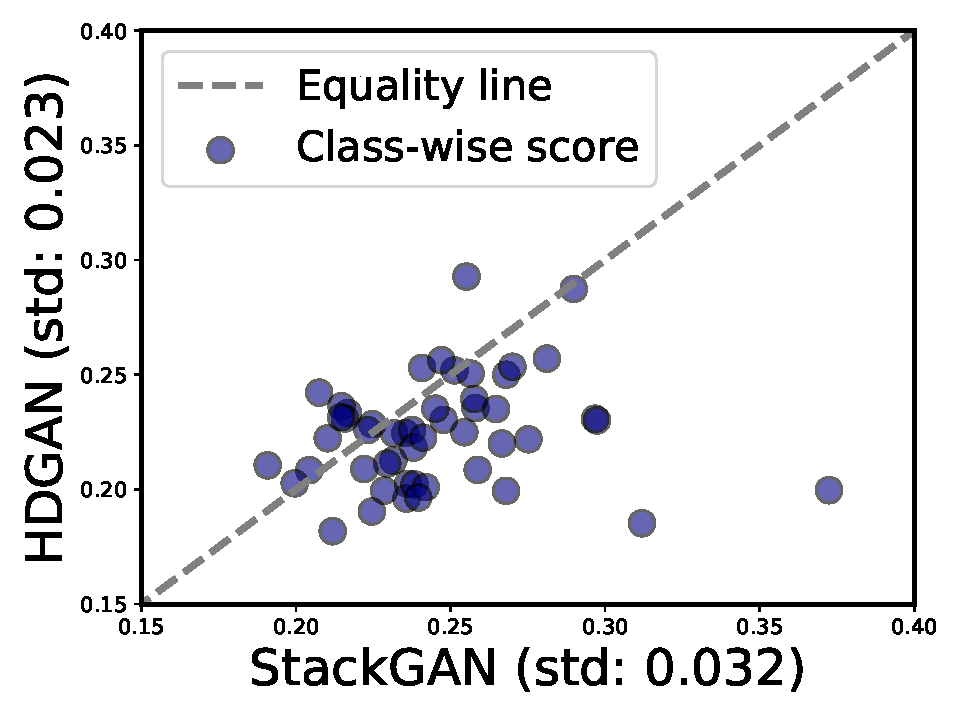
\includegraphics[width=0.99\textwidth,height=0.7\textwidth]{figure/ms_ssmi.pdf}
		\vspace{-1.8cm}
	\end{minipage} %\hfill
	\begin{minipage}[b]{0.49\linewidth}
		\begin{tabularx}{.9\textwidth}{c|c}
			\specialrule{1.5pt}{0pt}{0pt}  
			Method   &  MS-SSMI \\ \hline
			StackGAN &   0.234   \\ 
			Prog.GAN &   0.225    \\ \hline
			HDGAN    &   \textbf{0.215}    \\
		\end{tabularx}
	\end{minipage}
	\vspace{0.2cm}
	\caption{Left: Class-wise MS-SSMI evaluation. Lower score indicates higher intraclass invariance. The points below the equality line represent classes our HDGAN wins. Right: Overall (no class-wise) score evaluation.} \label{fig:msssmi}
\end{table}


\subsection{Comparative Results}
To validate our method, we compare our results with GAN-INT-CLS \cite{reed2016generative}, GAWWN \cite{reed2016learning}, TAC-GAN \cite{dash2017tac}, StackGAN \cite{han2017stackgan} and also its improved version StackGAN++ \cite{}, and Progressive GAN \cite{} \footnote{Note that StackGAN++ and Prog.GAN are two very recent released pre-prints we noticed before submission. We acknowledge them as they also target at generating high resolution images, in spite of their differences in motivations and network and training designs from ours. }

% Similarly with our HDGAN, it now can train $64{-}256$ directly. Each generator still take images from the bottom generator and supervised by a discriminator. Differently, our network is more like a simple Vanilla network (or a pure inverse ImageNet CNN).}. 

%StackGAN \cite{han2017stackgan} generates synthetic images up to $256{\times}256$ resolution. We show that our method can generates images up to $512{\times}512$.

Table \ref{table:score} shows the quantitative evaluation. HDGAN achieves significantly improvement compared to other methods. For example, HDGAN improves GAN-INT-CLS by ${\sim}30.1\%$  and ${\sim}8.4\%$ on CUB.

Table \ref{table:multiscales} quantitatively compares the the multi-resolution inception score. Our results are from the side outputs of a single model. Usually higher resolution images gives rise to better inception score since they contain details. As can be observed, our $64^2$ images outperforms $128^2$ images of StackGAN and our $128^2$ images outperforms $256^2$ images of StackGAN substantially. 

Table \ref{fig:msssmi} shows the MS-SSMI image quality evaluation score compared with StackGAN and ProgressiveGAN. StackGAN and our HDGAN use the semantic text as input so the generated images retain class information. We compare the score with StackGAN using the provided pretrained model). We randomly sample ${~}20,000$ image pairs (400 per class) and show the class-wise score in the left figure. HDGAN shows better performance in majority of classes and also has lower inter-class standard divition (0.023 vs. 0.032).
Prog.GAN takes noises rather than text. Since MS-SSMI evaluates the image quality without text or class involvement, we can compare with it. Following the procedure of Prog.GAN, we randomly sample ${~}10,000$ image pairs for each comparing method (For Prog.GAN, we use generated $256^2$ images provided by the author) and show the results in the right table. Our method outperforms both StackGAN and Prog.GAN. 



\subsubsection{Style Transfer Using Sentence Interpolation}

Ideally, a trained model should learn a smooth linear latent manifold of the images. To demonstrate our model's generalization capability, we generate images using the linearly interpolated  embedding using two source sentences. During this experiment, we fix the all the random noises to make the object and background consistent. As is shown in Figure~\ref{}, the generated images show gradual and smooth changes reflecting the semantic changing in sentences, while still maintaining plausible object pose and shape. In the first row, the generated birds gradually turn the color from red to yellow, in the second row, more complicated sentences containing more detailed appearance information (e.g., blue peaks, and yellow wing) are used, we can see that our model is still be able to successfully capture these subtle information and tune the bird appearance gradually. 

We also evaluate some sentences that generated by ourself, the resulting images are shown in Figure~\ref{}, as we can see, our model are robust and generalize well to human descriptions that never seen before. 


\subsubsection{What role does noise play}
In our model, there are two kinds of randomness injected to the input of the Generator, ie, epsilon $\epsilon$ and Gaussian noise vector $z$.
In this experiment, we fix the sentence embedding and one noise, and change the other random variable. For each random noise, we generate 4 different values. So In total 16 images are generated using all noise combinations, the resulting images are shown in Figure~\ref{}, $\epsilon$ and $z$ corresponds to row and column dimension, respectively. As is shown in the image, we can see that, $\epsilon$ can change the pose of the image, while $z$ is mainly responsible for the background variations. This clearly demonstrate that, our model learns to disentangle the semantic information from the pose and background information.

\section{On the effects of Individual Components}
\subsection{Hierarchically-nested adversary}
Recall that the proposed hierarchically-nested adversarial supervision plays a role of regularizing the layer representations. In practice, we apply it on feature maps at $\{64, 128, 256\}$. In Table \ref{table:deep-nest}, we show the inception score by removing partial of supervision components. As can be observed, ...

StackGAN emphasizes the importance of using text embeddings in the (stage-II) mid-level features of the $256{\times}256$ generator by showing an large drop from $3.7$ to $3.45$ without doing so. The text embedding plays an important role in maintaining the diversity and semantic consistency in StackGAN. While in our method, we only use text embeddings at the input. Our improved results demonstrate that our hierarchically-nested adversarial supervision regularizes the generator to achieve the same goal. 


\subsection{On the Local Image Loss}
\begin{table}[t] % retrieval
	\label{tab:local_loss}
	\begin{center}
		\begin{tabularx}{.32\textwidth}{c|cc}
			\specialrule{1.5pt}{0pt}{0pt}  
			Scale 						&   No Local 	& With Local				\\ 				\hline
			$64{\times}64$              &   ${2.95{\pm}.02}$       &  	$\bm{3.46{\pm}.04}$ \\
			$256{\times}256$             &   $3.70{\pm}.04$     &	$\bm{4.01{\pm}.06}$ \\ \hline
		\end{tabularx}
	\end{center} \vspace{-.4cm}
	\caption{Multi-scale inception score comparison. See text for explanation.} \label{table:multiscales}
\end{table}

We also study the effectiveness of the proposed local image loss. We conduct experiments with using architecture with side output 64$\times$64 and 256 $\times$ 256. 
As can be seen in Table\ref{tab:local_loss}, we can see that by removing local image loss (denoted as "No Local"), the inception score drop from \textcolor{red}{4.27} to \textcolor{red}{3.8}. To quantitatively compare the results, we also show generated results using two model in Figure \ref{local_or_not}, We can see that, also both models can successfully capture the semantic correspondence between image and sentence, 256$\times$ 256 results generated by model trained with local image loss provide more details, thus improving the visual quality.

\begin{figure}[t]
	\centering
	%	\includegraphics[width=0.48\textwidth]{}
	\caption{} \label{fig:vallina-res}
\end{figure}


\begin{table}[t] % retrieval
	\begin{center}
		\begin{tabularx}{.268\textwidth}{ccc|c}
			\specialrule{1.5pt}{0pt}{0pt}  
			\multicolumn{3}{c|}{Components}	&  \multirow{2}{*}{Score}	\\ \cline{1-3}
			64	& 128	& 256 			& 		\\ \hline
			&  		&	\checkmark	&	${3.52{\pm}.04}$	\\ 
			&  	\checkmark	&	\checkmark	&		\\
			\checkmark	&  			&	\checkmark	&  ${4.14{\pm}.03}$		\\
			\checkmark	&  \checkmark		&	\checkmark	&	${4.01{\pm}.04}$ \\
			
		\end{tabularx}
	\end{center} \vspace{-.4cm}
	\caption{Ablation study for hierarchically-nested adversarial supervision.} \label{table:deep-nest}
\end{table}

\subsection{Design principles}
Note that for text-to-image synthesis, StackGAN is the only successful method to generate $256{\times}256$ images.
At the same time, it also shows the difficulty (impossibility) of directly training a vanilla $256{\times}256$ GAN, which fails to generate meaningful images. 
We test this extreme case using our method by removing all nested supervisions (the first row of Table \ref{table:deep-nest}). Our method still generates fairly good results. Figure \ref{fig:vallina-res} shows the qualitatively results. This strongly proves the effectiveness of our designs in generators and discriminator losses.

Initially, we tried to share top layers of the hierarchical discriminators of HDGAN inspired by \cite{liu2017unsupervised} with an intuition to reduce their variances and unify their common goal (i.e. differentiates real and fake despite difficult scales). However, we did not find any benefits from this and our independent discriminators can be well-trained by themselves. 

\textbf{Advantages}
The advantages of our hierarchical-nested adversary are clearer from different views, compared with the popular stacking GAN strategy \cite{}. 

First, it is memory efficient. 
When viewing it as ensembled multi-scale GAN (Figure \ref{}), each GAN fully uses the parameters of its lower resolution GAN. Usually, a deeper generator is necessary to compact a discriminator. Since the depth of discriminator increases as image resolution increases, if stacking separate GANs based on low resolution GAN outputs, much more layers are needed in generators as wells. While in our method, for instance, from a $64^2$ GAN to a $128^2$ GAN, only a minimum two conv layers ($1$-repeat res-blocks) are needed. 

Second, it fully enjoys top-down knowledge. 
The low resolution can not use high resolution information in the stacking GAN strategy. While in our method, it is easy to see the low resolution GAN enjoys knowledge from higher resolution. As an evidence, our $64^2$ synthetic images have higher inception score than $64^2$ and even $128^2$ images of StackGAN (see Section 5).


\section{Conclusion}
...

{\small
\bibliographystyle{ieee}
\bibliography{reference_zizhao,egbib}
}

\end{document}
